\section{Сравнение конфигураций}

\subsection{Сравнение аппроксимаций}
\begin{itemize}
    \item \textbf{$q_1$ (full)}: лучшая точность, наиболее устойчивый baseline для этой задачи.
    \item \textbf{$q_2$ (diagonal)}: чуть хуже, но близка к $q_1$ и проще в интерпретации.
    \item \textbf{$q_3$ (FD Hessian)}: хуже на текущих настройках, требует отдельного sweep по $\epsilon$.
\end{itemize}

\subsection{Сравнение по осям 1D-среза}
\begin{figure}[H]
    \centering
    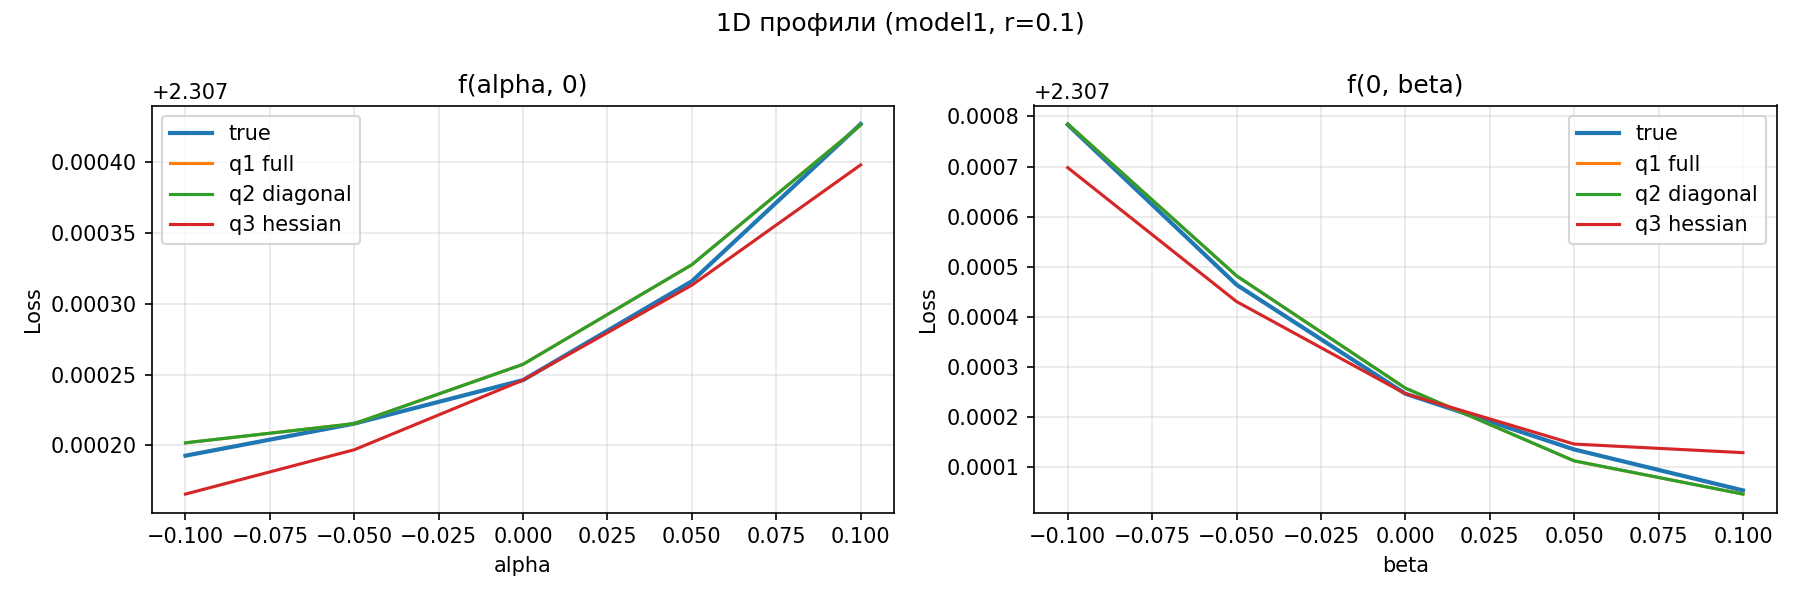
\includegraphics[width=0.9\textwidth]{figures/profile_1d_model1_r0.1.png}
    \caption{Срезы $f(\alpha,0)$ и $f(0,\beta)$ и их аппроксимации.}
    \label{fig:profile_1d}
\end{figure}

\subsection{Что не добавлялось сознательно}
Confusion matrix, ROC-кривые и другие классификационные визуализации не включены, поскольку они не являются центральными для цели ЛР (исследование геометрии loss landscape, а не сравнение классификаторов по precision/recall).
